%%%%%%%%%%%%%%%%%%%%%%%%%%%%%%%%%%%%%%%%%%%%%%%%%%%%%%%%%%%%%%%%%%%%%%
% LaTeX Template: Curriculum Vitae
%
% Source: http://www.howtotex.com/
% Feel free to distribute this template, but please keep the
% referal to HowToTeX.com.
% Date: July 2011
%Version for spanish users, by dgarhdez
% 
%%%%%%%%%%%%%%%%%%%%%%%%%%%%%%%%%%%%%%%%%%%%%%%%%%%%%%%%%%%%%%%%%%%%%%
% How to use writeLaTeX: 
%
% You edit the source code here on the left, and the preview on the
% right shows you the result within a few seconds.
%
% Bookmark this page and share the URL with your co-authors. They can
% edit at the same time!
%
% You can upload figures, bibliographies, custom classes and
% styles using the files menu.
%
% If you're new to LaTeX, the wikibook is a great place to start:
% http://en.wikibooks.org/wiki/LaTeX
%
%%%%%%%%%%%%%%%%%%%%%%%%%%%%%%%%%%%%%%%%%%%%%%%%%%%%%%%%%%%%%%%%%%%%%%
\documentclass[paper=a4,fontsize=11pt]{scrartcl} % KOMA-article class

\usepackage[spanish]{babel}
\usepackage[utf8x]{inputenc}
\usepackage[protrusion=true,expansion=true]{microtype}
\usepackage{amsmath,amsfonts,amsthm}     % Math packages
\usepackage{graphicx}                    % Enable pdflatex
\usepackage[svgnames]{xcolor}            % Colors by their 'svgnames'
\usepackage{geometry}
	\textheight=675px                    % Saving trees ;-)
\usepackage{url}

\frenchspacing              % Better looking spacings after periods
\pagestyle{empty}           % No pagenumbers/headers/footers

%%% Custom sectioning (sectsty package)
%%% ------------------------------------------------------------
\usepackage{sectsty}

\sectionfont{%			            % Change font of \section command
	\usefont{OT1}{phv}{b}{n}%		% bch-b-n: CharterBT-Bold font
	\sectionrule{0pt}{0pt}{-4pt}{1pt}}

%%% Macros
%%% ------------------------------------------------------------
\newlength{\spacebox}
\settowidth{\spacebox}{888888888}			% Box to align text
\newcommand{\sepspace}{\vspace*{0.1mm}}		% Vertical space macro

\newcommand{\MyName}[1]{ % Name
		\Huge \usefont{OT1}{phv}{b}{n} \hfill #1
		\par \normalsize \normalfont}
		
\newcommand{\MySlogan}[1]{ % Slogan (optional)
		\large \usefont{OT1}{phv}{m}{n}\hfill \textit{#1}
		\par \normalsize \normalfont}

\newcommand{\NewPart}[1]{\section*{\uppercase{#1}}}

\newcommand{\PersonalEntry}[2]{
		\noindent\hangindent=2em\hangafter=0 % Indentation
		\parbox{\spacebox}{        % Box to align text
		\textit{#1}}		       % Entry name (birth, address, etc.)
		\hspace{1.5em} #2 \par}    % Entry value

\newcommand{\SkillsEntry}[2]{      % Same as \PersonalEntry
		\noindent\hangindent=2em\hangafter=0 % Indentation
		\parbox{\spacebox}{        % Box to align text
		\textit{#1}}			   % Entry name (birth, address, etc.)
		\hspace{1.25em} #2 \par}    % Entry value	
		
\newcommand{\EducationEntry}[4]{
		\noindent \textbf{#1} \hfill      % Study
		\colorbox{White}{%
			\parbox{5cm}{%
			\hfill\color{Black}#2}} \par  % Duration
		\noindent \textit{#3} \par        % School
		\noindent\hangindent=2em\hangafter=0 \small #4 % Description
		\normalsize \par}

\newcommand{\WorkEntry}[4]{				  % Same as \EducationEntry
		\noindent \textbf{#1} \hfill      % Jobname
		\colorbox{White}{%
			\parbox{5cm}{%
			\hfill\color{Black}#2}} \par  % Duration
		\noindent \textit{#3} \par              % Company
		\noindent\hangindent=2em\hangafter=0 \small #4 % Description
		\normalsize \par}

%%% Begin Document
%%% ------------------------------------------------------------
\begin{document}
% you can upload a photo and include it here...
%\begin{wrapfigure}{r}{0.5\textwidth}
%	\vspace*{-2em}
%		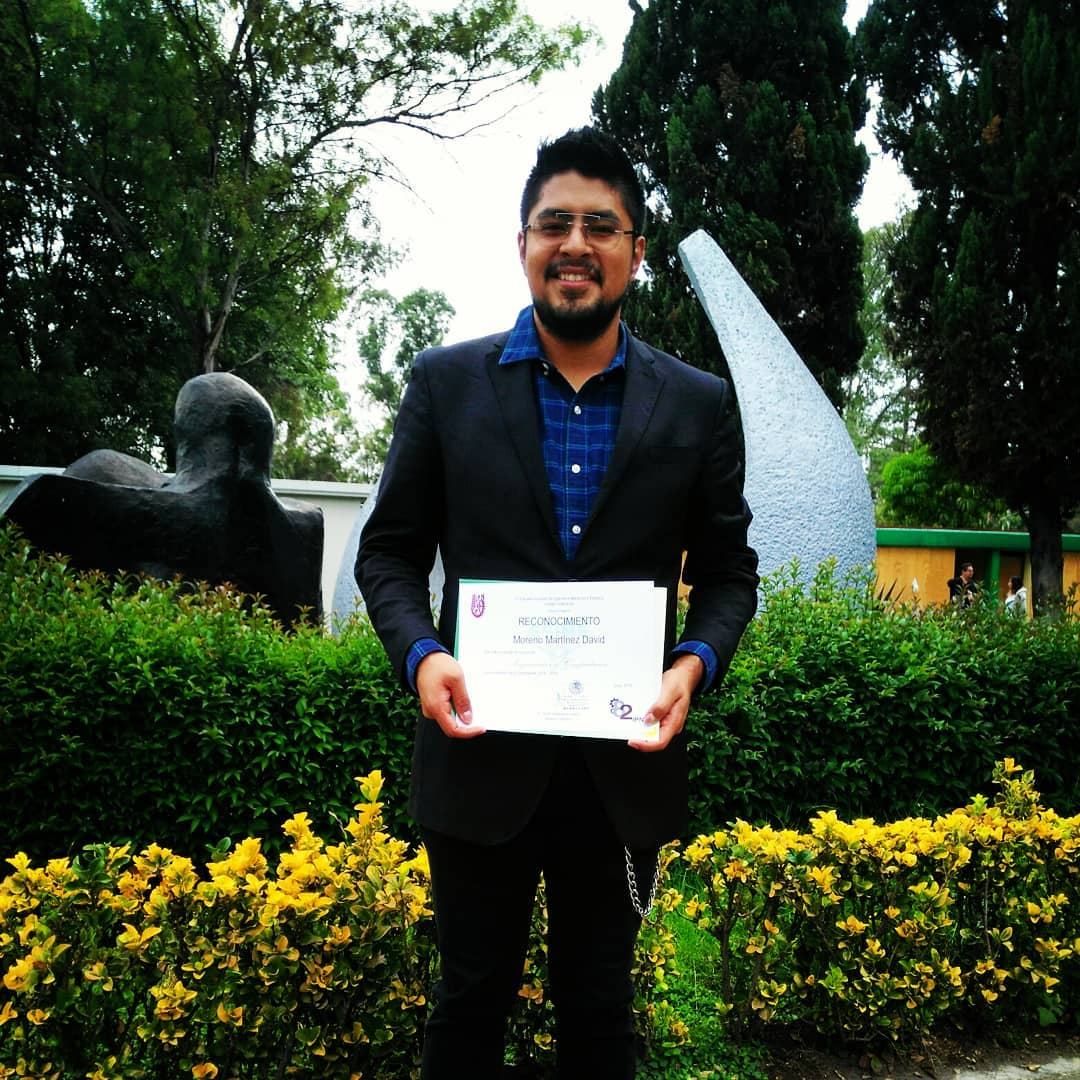
\includegraphics[width=0.15\textwidth]{dave.jpg}
%\end{wrapfigure}

\MyName{David Moreno Martínez}
\MySlogan{Ingeniero en Computación}

\sepspace

%%% Personal details
%%% ------------------------------------------------------------
\NewPart{Datos personales}{}

\PersonalEntry{Nacimiento}{25 de agosto de 1995}
\PersonalEntry{Teléfono}{(55) 57-42-02-12}
\PersonalEntry{Celular}{(+52) 044-55-4801-0062}
\PersonalEntry{E-Mail}{\url{dmorenom1403@alumno.ipn.mx}}

%%% Education
%%% ------------------------------------------------------------
\NewPart{Educación}{}

\EducationEntry{Ingeniería en Computación (Título en trámite)}{2014-2018}{Escuela Superior de Ingeniería Mecánica y Eléctrica Unidad Culhuacán}{
\begin{itemize}
\item{Proyecto de fin de carrera: \emph{Modelado y Simulación por HID de un brazo robótico en Realidad Aumentada}}
\end{itemize}
}

\NewPart{Cursos Extracurriculares}{}

\EducationEntry{Programación en Java}{2016}{En Línea}{}

\sepspace

\EducationEntry{Programación en Python}{2017}{En Línea}{}

\sepspace

\EducationEntry{Ingeniería de Software}{2017}{IPN}{}

\sepspace

\EducationEntry{Bases de Datos en Oracle}{2017}{IPN}{}

\sepspace

\EducationEntry{Curso de Android Studio}{2017}{En Línea}{}

\sepspace

\EducationEntry{PHP Orientado a Objetos}{2018}{En Línea}{}

\sepspace

\EducationEntry{Bases de Datos en MySQL}{2018}{IPN}{}

\sepspace

\EducationEntry{Curso de Java EE}{2018}{En Línea}{}

\sepspace

\EducationEntry{Desarrollo Web Full-Stack}{2018}{Kodemia}{}

%%% Work experience
%%% ------------------------------------------------------------
\NewPart{Experiencia}

\WorkEntry{Project Manager Junior}{Marzo 2017}{AutoClean Express}{
\begin{itemize}
\item{Realización de Plan de Negocios para mantenimiento y mejora de la aplicación de la empresa.}
\end{itemize}
}

\WorkEntry{Desarrollador RA (Realidad Aumentada)}{Mayo 2017 - Junio 2018}{IPN}{
\begin{itemize}
\item{Desarrollo de una aplicación tipo simulador implementando Realidad Aumentada para el manejo y presentación de maquinaria pesada en la industria metal-mecánica.}
\end{itemize}
}
\sepspace

\WorkEntry{Soporte Técnico}{2018 - Actualidad}{Independiente}{
\begin{itemize}
\item{Configuración de computadoras, impresoras, scaner's, modems.}
\end{itemize}
}

%%% Skills
%%% ------------------------------------------------------------
\NewPart{Conocimientos y Habilidades (Skills)}

\SkillsEntry{Aptitudes}{}
\SkillsEntry{}{Autodidacta}
\SkillsEntry{}{Cacapidad de Organización}
\SkillsEntry{}{Buen Negociador}
\SkillsEntry{}{Trabajo en equipo}
\SkillsEntry{}{Flexibilidad y adaptación a cambios}
\SkillsEntry{}{Análisis y resolución de problemas}

\SkillsEntry{Idiomas}{}
\SkillsEntry{}{Español (Nativo)}
\SkillsEntry{}{Inglés (Avanzado)(70\%)}

\SkillsEntry{Técnicas/os}{}
\SkillsEntry{}{Microsoft Office, Visio, Project}
\SkillsEntry{}{Corel Draw, AutoCAD, SolidWorks, Unity, Blender}
\SkillsEntry{}{Manejo de repositorios con Git y GitHub}
\SkillsEntry{}{Conocimiento sobre contenedores Docker}
\SkillsEntry{}{Conocimiento y manejo en Virtual Machines}
\SkillsEntry{}{Manejo de documentación y diagramas UML}
\SkillsEntry{}{Conocimiento en varios IDE's y Editores de código}
\SkillsEntry{}{Configuración de Computadoras Windows/Linux}
\SkillsEntry{}{Configuración de impresoras/scaner's}
\SkillsEntry{}{Conocimiento de redes de computadoras}
\SkillsEntry{}{Assembler 8086, C/C++, Java, Python, C\#, VB .NET}
\SkillsEntry{}{PHP, Javascript, MySQL, HTML5, XML, CSS3, Ruby, Perl}
\SkillsEntry{}{Django, Flask, React, Ionic, Node.js}
\SkillsEntry{}{Bootstrap, jQuery, Laravel}
%\SkillsEntry{}{}

%%% References
%%% ------------------------------------------------------------
%\NewPart{References}{}
%Available upon request
\end{document}
